\documentclass{article}
\usepackage[final]{nips_2017}
\usepackage[polish]{babel}
\usepackage[utf8]{inputenc} % allow utf-8 input
\usepackage[T1]{fontenc}    % use 8-bit T1 fonts
\usepackage{hyperref}       % hyperlinks
\usepackage{url}            % simple URL typesetting
\usepackage{booktabs}       % professional-quality tables
\usepackage{amsfonts}       % blackboard math symbols
\usepackage{nicefrac}       % compact symbols for 1/2, etc.
\usepackage{microtype}      % microtypography
\usepackage{graphicx}
\usepackage[section]{placeins}
\graphicspath{ {./images/} }

\title{ Sieć wielowarstwowa uczona metodą propagacji wstecznej  }

\author{
  Autor: Rafał Behrendt \\
  \texttt{246643@student.pwr.edu.pl} \\
  Prowadząca: dr hab. inż. Urszula Markowska-Kaczmar \\
  \today
}

\begin{document}

\maketitle

\begin{abstract}
  Celem ćwiczenia jest zapoznanie się technikami poprawiającymi szybkość uczenia sieci. Eksperymenty przeprowadzono na zbiorze
  MNIST zawierającym 60000 danych treningowych oraz 10000 danych testowych. Każdy test przeprowadzono 10 razy, a wyniki uśredniono.
\end{abstract}

Kod źródłowy znajduje się w poniższym linku:

\begin{center}
  \url{https://github.com/aspirew/neuralNetworks/tree/list3}
\end{center}

\newpage
\section{Eksperymenty}

Za domyślne hiperparametry przyjęto:

\begin{itemize}
  \item Wielkość sieci: [20]
  \item Współczynnik uczenia: 0.01
  \item Inicjalizacja wag za pomocą rozkładu normalnego o parametrach:
  \subitem mi: 0
  \subitem sigma: 0.1
\end{itemize}

Każdy test przeszedł przez 50 epok zanim został zakończony.

\section{Test optymalizatorów współczynnika uczenia}

Zbadano jak podane w ćwiczeniu optymaliztory wpływają na skuteczność i szybkość uczenia. Wyniki działania optymalizatorów porównano
z wnikami bez ich użycia. Optymaliztory przetestowano na dwóch funkcjach aktywacji: sigmoidalnej i ReLU. W
tabelach zawarte są uśrednione błędy oraz oraz uśredniona liczba prawidłowo rozpoznanych liczb ze
zbioru testowego. Niżej przedstawione są wyniki na wykresach

\subsection{Funkcja sigmoidalna}

\begin{table}[h]
  \centering
    
  \bgroup
  \def\arraystretch{1.3}
\begin{tabular}{|l|l|l|}
\hline
Optymalizator & Błąd & Skuteczność \\ \hline
Brak & 1.43 & 6649.3 \\ \hline
Momentum & 0.81 & 7923 \\ \hline
Momentum Nesterova & 0.81 & 7956.9 \\ \hline
Adagrad & 0.91 & 7583.8 \\ \hline
Adadelta & 0.83 & 7764.9 \\ \hline
Adam & 0.65 & 7946.4 \\ \hline
\end{tabular}
  \egroup
  \vspace{10pt}
  \caption{Optymalizatory - funkcja sigmoidalna}
\end{table}

\newpage

\begin{figure}[!htb]
  \centering
  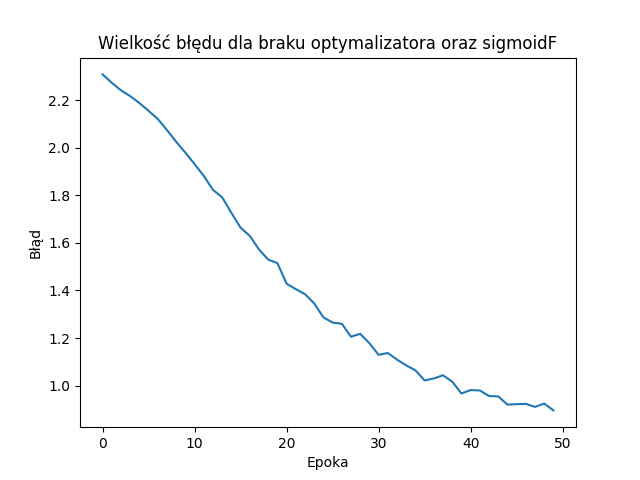
\includegraphics[width=\linewidth]{error_none_sigmoidF.png}
\end{figure}

\begin{figure}[!htb]
  \centering
  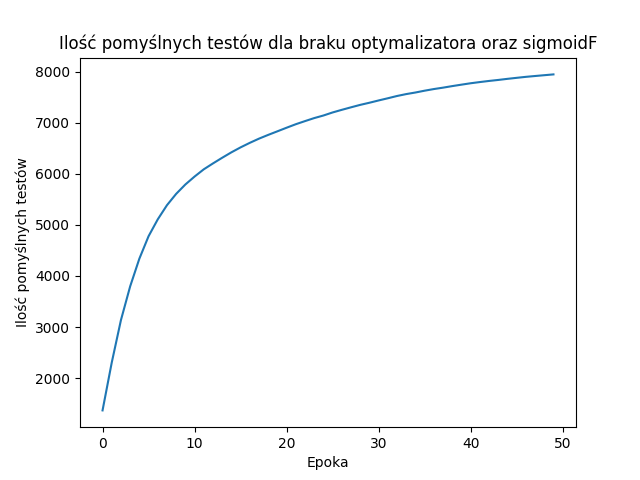
\includegraphics[width=\linewidth]{test_none_sigmoidF.png}
\end{figure}

W przypadku braku optymalizatora można zauważyć, że wykres błędu zmniejsza się powoli, a sam średni błąd jest
na wysokim poziomie.

\begin{figure}[!htb]
  \centering
  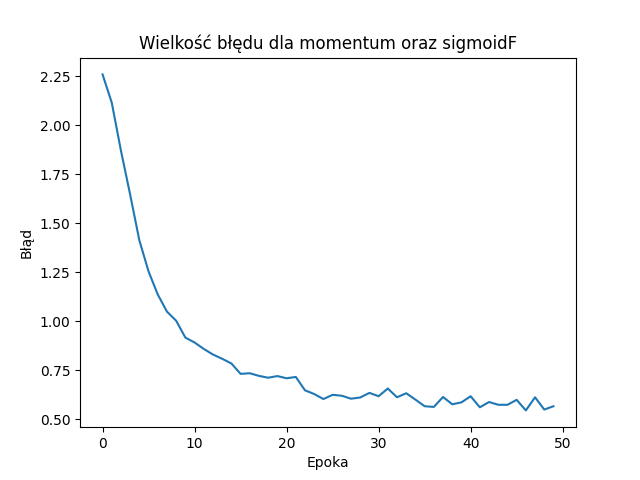
\includegraphics[width=\linewidth]{error_momentum_sigmoidF.png}
\end{figure}

\begin{figure}[!htb]
  \centering
  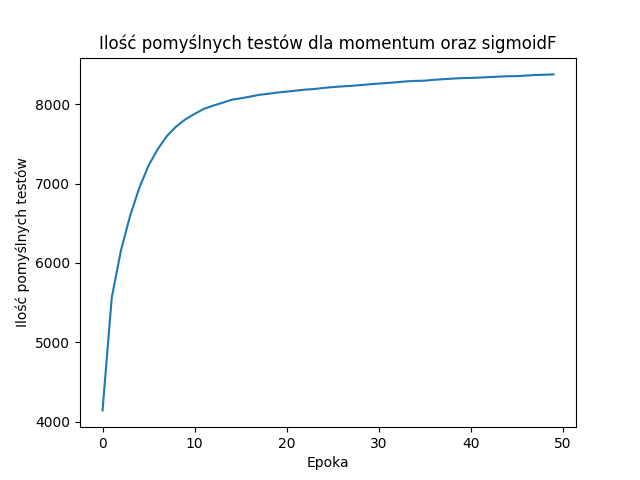
\includegraphics[width=\linewidth]{test_momentum_sigmoidF.png}
\end{figure}

Metoda momentum wyraźnie zwiększa szybkość uczenia sieci - wykres szybciej schodzi do optimum. Ilość pomyślnych testów
jest na podobnym poziomie jak przy braku optymalizatora, jednak graniczna wartość osiągnięta jest znacznie szybciej.

\begin{figure}[!htb]
  \centering
  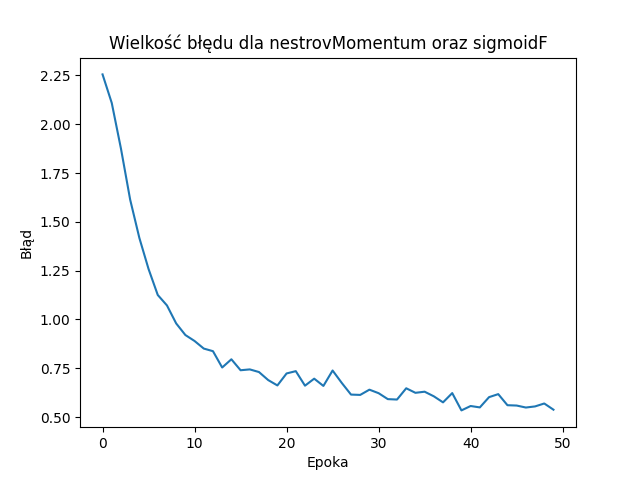
\includegraphics[width=\linewidth]{error_nestrovMomentum_sigmoidF.png}
\end{figure}

\begin{figure}[!htb]
  \centering
  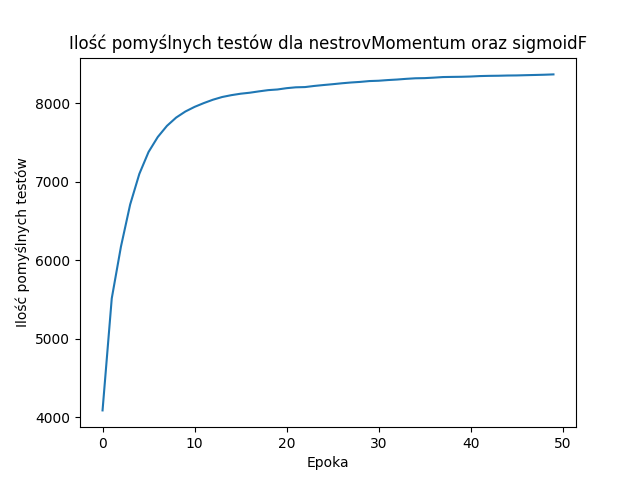
\includegraphics[width=\linewidth]{test_nestrovMomentum_sigmoidF.png}
\end{figure}

Momentum Nesterova daje zbliżone wyniki jak zwykłe momentum - ponownie widać poprawę względem braku optymalizatora.

\begin{figure}[!htb]
  \centering
  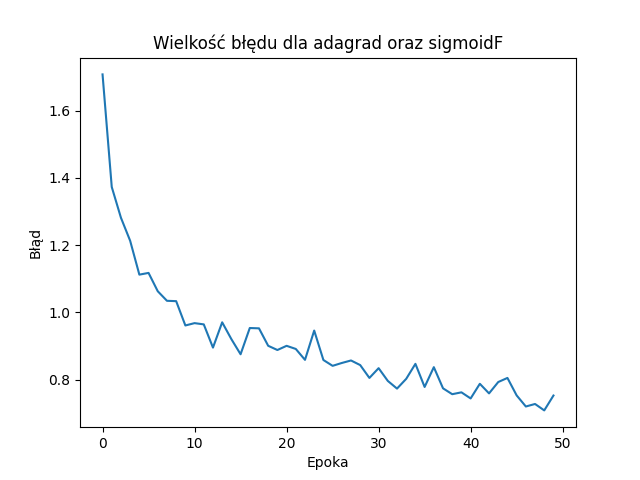
\includegraphics[width=\linewidth]{error_adagrad_sigmoidF.png}
\end{figure}

\begin{figure}[!htb]
  \centering
  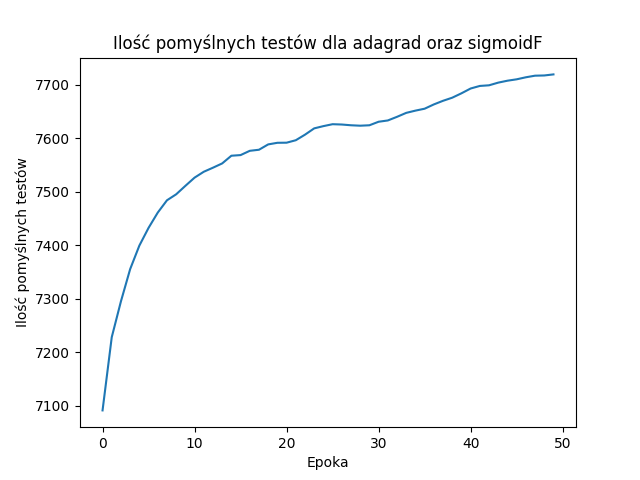
\includegraphics[width=\linewidth]{test_adagrad_sigmoidF.png}
\end{figure}

Optymalizator adagrad działa dość niestabilnie. Błąd spada szybciej niż w przypadku braku optymalizatora.

\begin{figure}[!htb]
  \centering
  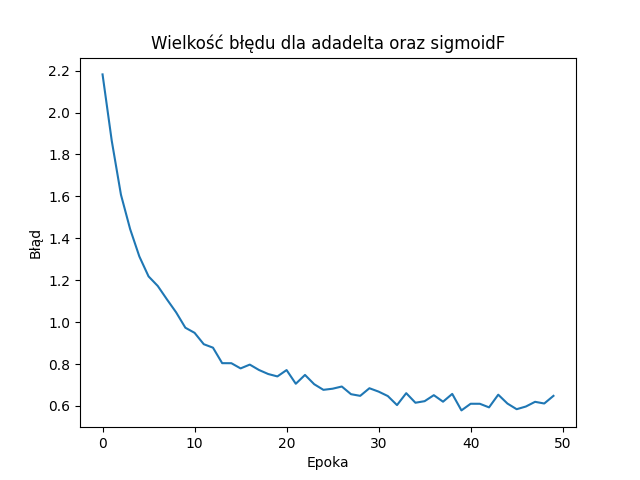
\includegraphics[width=\linewidth]{error_adadelta_sigmoidF.png}
\end{figure}

\begin{figure}[!htb]
  \centering
  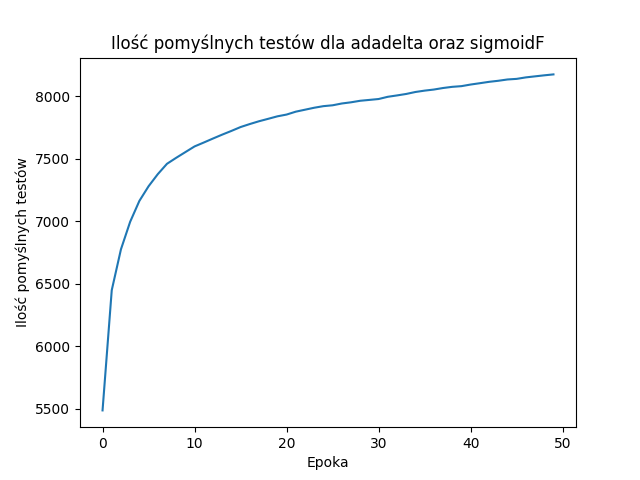
\includegraphics[width=\linewidth]{test_adadelta_sigmoidF.png}
\end{figure}

Ustabilizowanie można zauważyć w przypadku optymalizatora adadelta. Widać poprawę względem adagrad.

\begin{figure}[!htb]
  \centering
  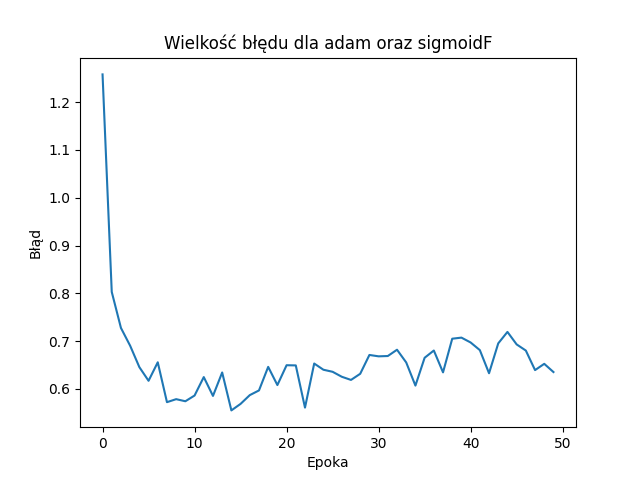
\includegraphics[width=\linewidth]{error_adam_sigmoidF.png}
\end{figure}

\begin{figure}[!htb]
  \centering
  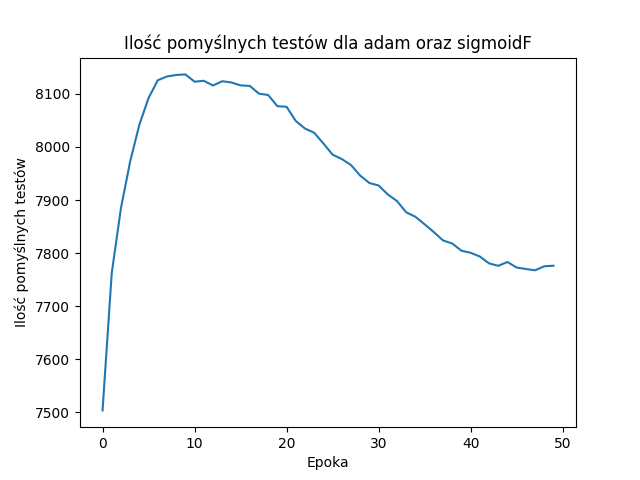
\includegraphics[width=\linewidth]{test_adam_sigmoidF.png}
\end{figure}

Optymalizator adam nie osiągnął najlepszej średniej wartości błędu. Na wykresie widać jednak, że osiąga on optimum zdecydowanie najszybciej - do tego stopnia że po 20 epoce
można zauważyć objawy przeuczenia się sieci, co skutkowało pogorszeniem średnich wyników.


\newpage
\subsection{Funkcja ReLU}

\begin{table}[h]
  \centering
    
  \bgroup
  \def\arraystretch{1.3}
  \begin{tabular}{|l|l|l|}
  \hline
  Optymalizator & Błąd & Skuteczność \\ \hline
  Brak & 0.6 & 8450.87 \\ \hline
  Momentum & 0.34 & 9104.6 \\ \hline
  Momentum Nesterova & 0.35 & 9109.2 \\ \hline
  Adagrad & 0.26 & 9276.0 \\ \hline
  Adadelta & 0.32 & 9174.3 \\ \hline
  Adam & 0.13 & 9526.7 \\ \hline
  \end{tabular} 
  \egroup
  \vspace{10pt}
  \caption{Optymalizatory - funkcja ReLU}
\end{table}

\newpage
\begin{figure}[!htb]
  \centering
  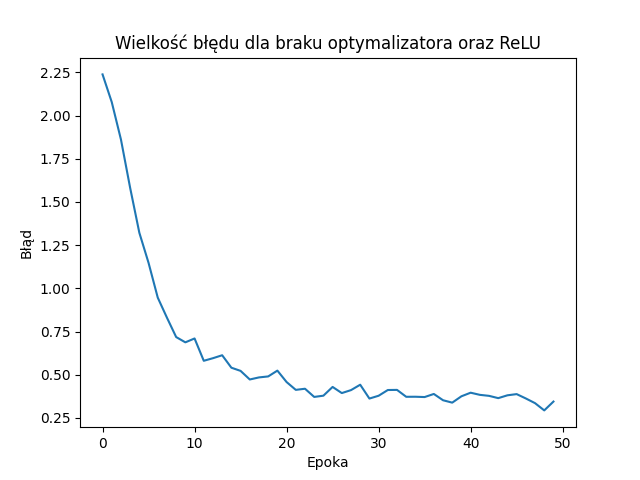
\includegraphics[width=\linewidth]{error_none_ReLU.png}
\end{figure}

\begin{figure}[!htb]
  \centering
  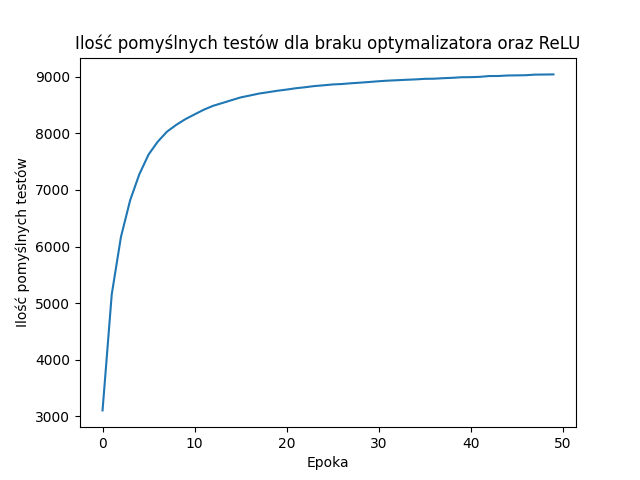
\includegraphics[width=\linewidth]{test_none_ReLU.png}
\end{figure}

Można zauważyć, że funkcja aktywacji ReLU radzi sobie lepiej niż funkcja sigmoidalna. Wykres szybciej osiąga 
optimum pomimo tego, że nie zastosowano żadnego optymalizatora.

\begin{figure}[!htb]
  \centering
  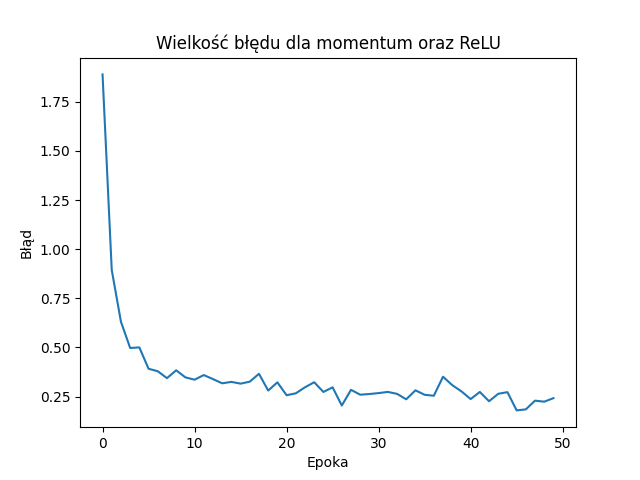
\includegraphics[width=\linewidth]{error_momentum_ReLU.png}
\end{figure}

\begin{figure}[!htb]
  \centering
  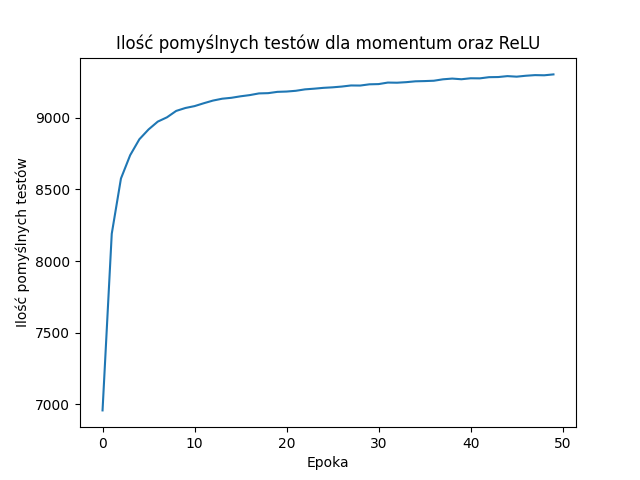
\includegraphics[width=\linewidth]{test_momentum_ReLU.png}
\end{figure}

Wydajność jest jeszcze lepsza, dzięki zastosowaniu momentum - wykres szybciej zbiega do optimum.

\begin{figure}[!htb]
  \centering
  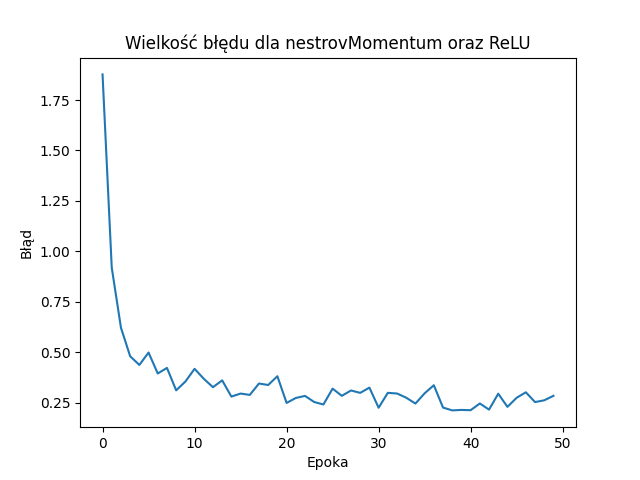
\includegraphics[width=\linewidth]{error_nestrovMomentum_ReLU.png}
\end{figure}

\begin{figure}[!htb]
  \centering
  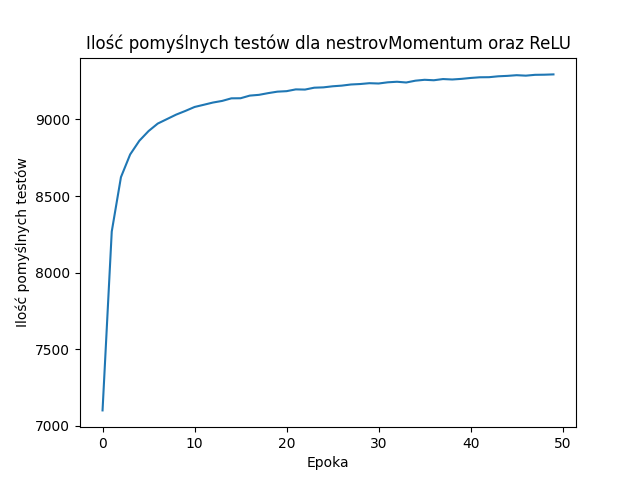
\includegraphics[width=\linewidth]{test_nestrovMomentum_ReLU.png}
\end{figure}

Ponownie momentum Nesterova prezentuje zbliżone wyniki do momentum.

\begin{figure}[!htb]
  \centering
  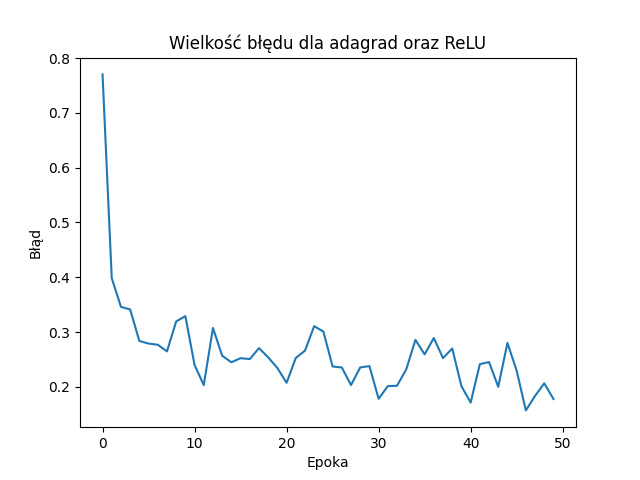
\includegraphics[width=\linewidth]{error_adagrad_ReLU.png}
\end{figure}

\begin{figure}[!htb]
  \centering
  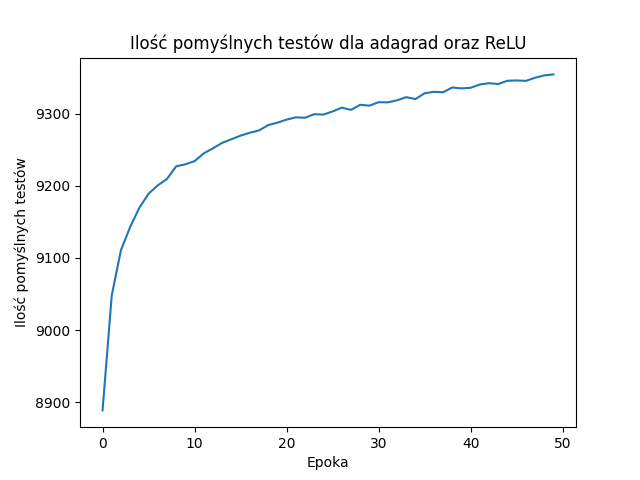
\includegraphics[width=\linewidth]{test_adagrad_ReLU.png}
\end{figure}

Jak w przypadku funkcji sigmoidalnej, tak i dla funkcji ReLU adagrad wyznacza się niestabilnością.

\begin{figure}[!htb]
  \centering
  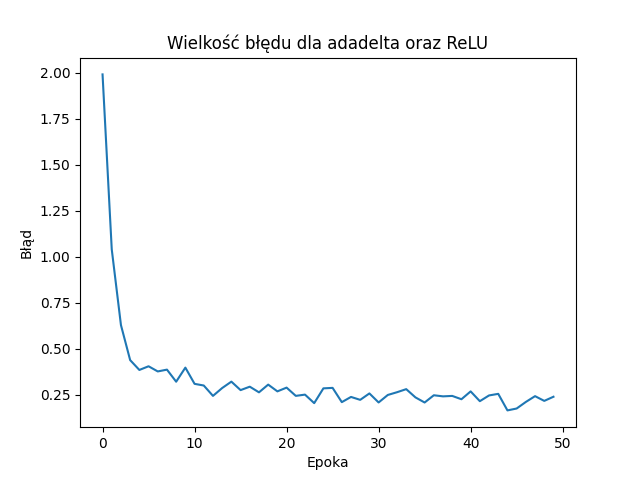
\includegraphics[width=\linewidth]{error_adadelta_ReLU.png}
\end{figure}

\begin{figure}[!htb]
  \centering
  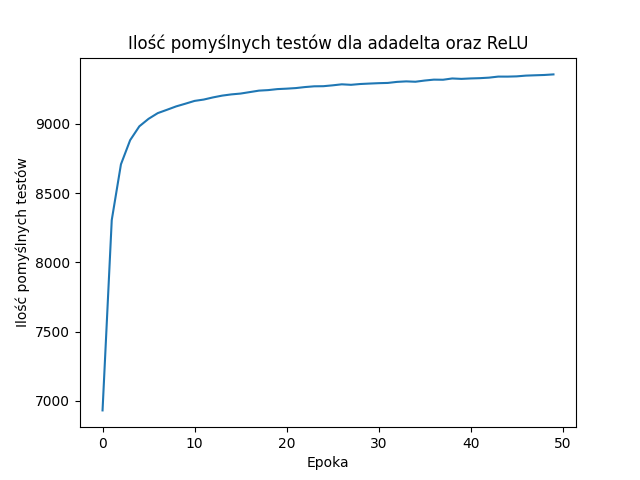
\includegraphics[width=\linewidth]{test_adadelta_ReLU.png}
\end{figure}

Adadelta szybko zbiega do optimum, a wykres jest bardziej stabilny niż to było w przypadku adagrad. Średnie wyniki są jednak gorsze - w odróżnieniu do funkcji sigmoidalnej.

\begin{figure}[!htb]
  \centering
  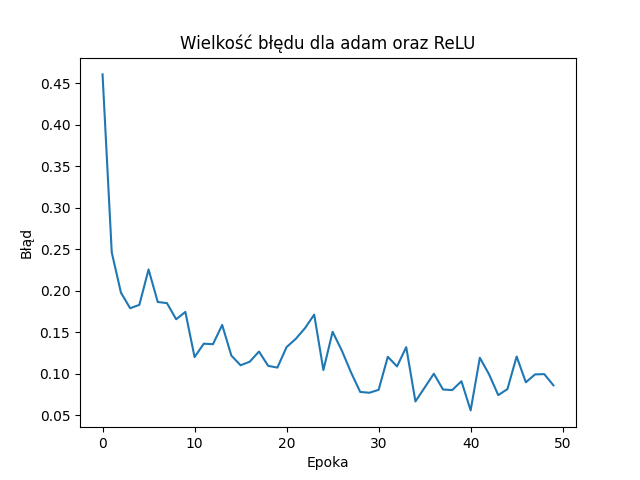
\includegraphics[width=\linewidth]{error_adam_ReLU.png}
\end{figure}

\begin{figure}[!htb]
  \centering
  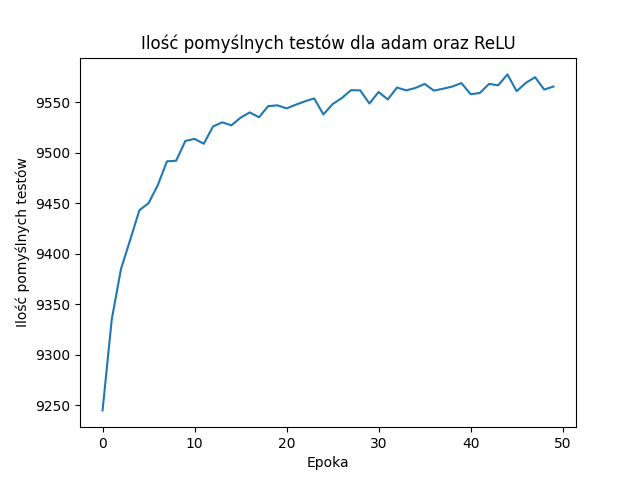
\includegraphics[width=\linewidth]{test_adam_ReLU.png}
\end{figure}

Wydawać by się mogło, że adam wykazuje się niestabilnością - wynika to jednak ze zmniejszonej skali, gdyż wyniki są wyjątkowo dobre.
Błąd rzędu 0.1 oraz skuteczność ponad 95\% pokazują skuteczność tego optymalizatora.

\newpage
\section{Inicjalizacja wag sieci}

Zbadano jak różne sposoby inicjalizacji wag w sieci wpływają na skuteczność i szybkość uczenia. 
Do optymalizacji nie użyto żadnego optymalizatora.
W tabelach zawarte są uśrednione błędy oraz oraz uśredniona liczba prawidłowo rozpoznanych liczb ze
zbioru testowego. Niżej przedstawione są wyniki na wykresach

\subsection{Funkcja sigmoidalna}

\begin{table}[h]
  \centering
    
  \bgroup
  \def\arraystretch{1.3}
  \begin{tabular}{|l|l|l|l|}
  \hline
  Metoda inicjalizacji & Błąd & Skuteczność \\ \hline
  Rozkład normalny $\sigma = 0.1$ & 1.43 & 6649.3 \\ \hline
  Xavier & 1.18 & 7416.43 \\ \hline
  He & 1.17 & 7543.632 \\ \hline
  \end{tabular}
  \egroup
  \vspace{10pt}
  \caption{Inicjalizacja wag - funkcja sigmoidalna}
\end{table}

\newpage
\begin{figure}[!htb]
  \centering
  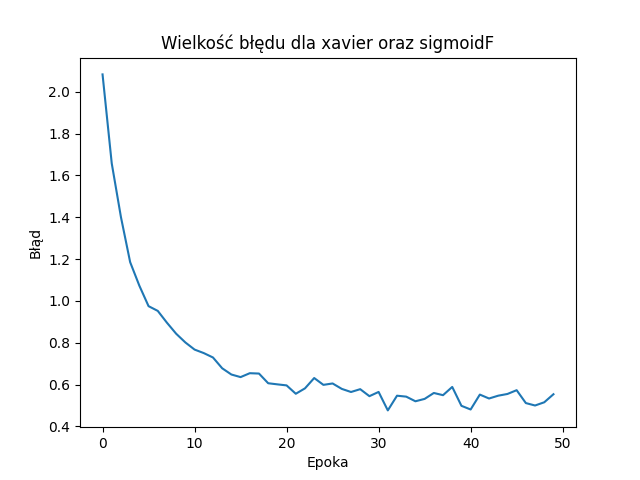
\includegraphics[width=\linewidth]{error_xavier_sigmoidF.png}
\end{figure}

\begin{figure}[!htb]
  \centering
  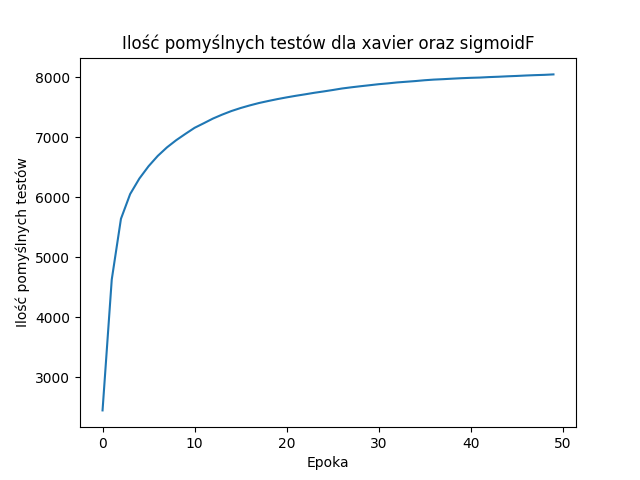
\includegraphics[width=\linewidth]{test_xavier_sigmoidF.png}
\end{figure}

Od razu można zauważyć, że prędkość oraz skuteczność znacząco rośnie w porównaniu do użycia samego rozkładu normalnego.

\newpage
\begin{figure}[!htb]
  \centering
  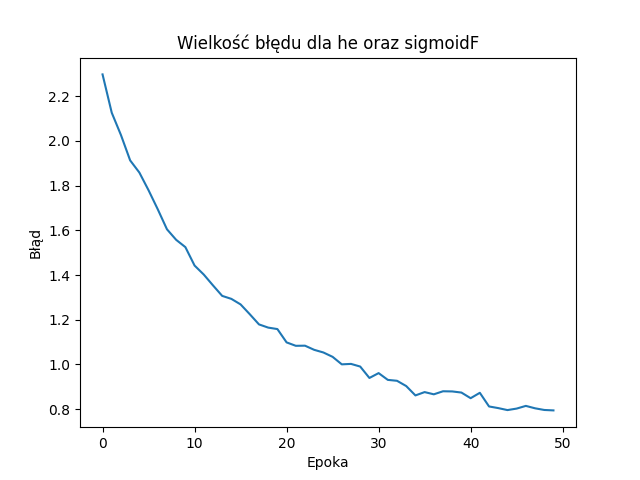
\includegraphics[width=\linewidth]{error_he_sigmoidF.png}
\end{figure}

\begin{figure}[!htb]
  \centering
  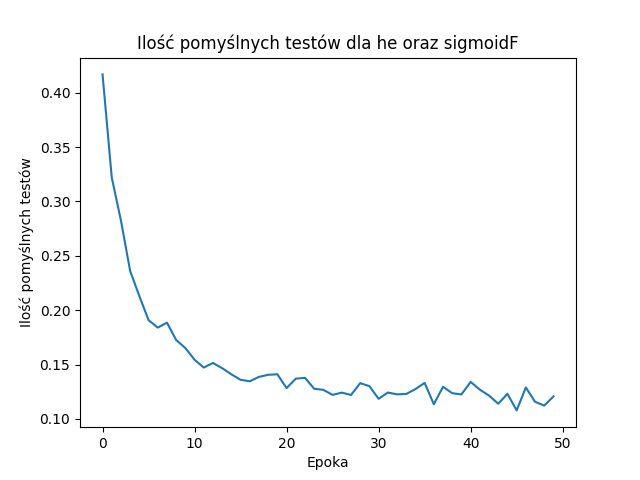
\includegraphics[width=\linewidth]{test_he_sigmoidF.png}
\end{figure}

Wyniki są zbliżone do metody xaviera - prędkość uczenia właściwie się nie zmienia, a skuteczność nieznacznie rośnie.

\newpage
\subsection{Funkcja ReLU}

\begin{table}[h]
  \centering
    
  \bgroup
  \def\arraystretch{1.3}
  \begin{tabular}{|l|l|l|l|}
  \hline
  Metoda inicjalizacji & Błąd & Skuteczność \\ \hline
  Rozkład normalny $\sigma = 0.1$ & 0.6 & 8450.87 \\ \hline
  Xavier & 0.48 & 8813.91 \\ \hline
  He & 0.48 & 8799.37 \\ \hline
  \end{tabular}
  \egroup
  \vspace{10pt}
  \caption{Inicjalizacja wag - funkcja ReLU}
\end{table}

\newpage
\begin{figure}[!htb]
  \centering
  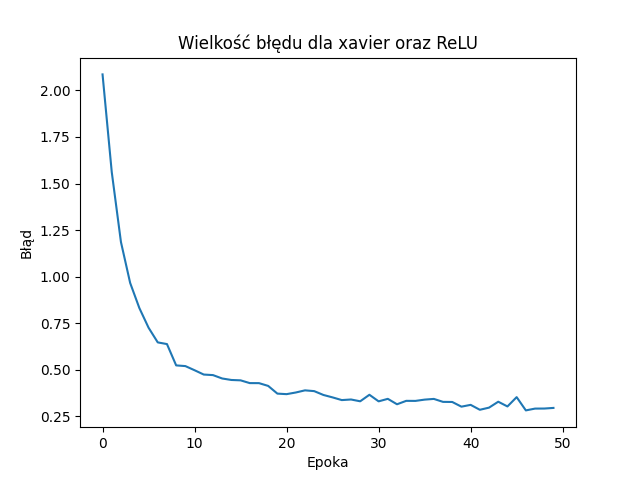
\includegraphics[width=\linewidth]{error_xavier_ReLU.png}
\end{figure}

\begin{figure}[!htb]
  \centering
  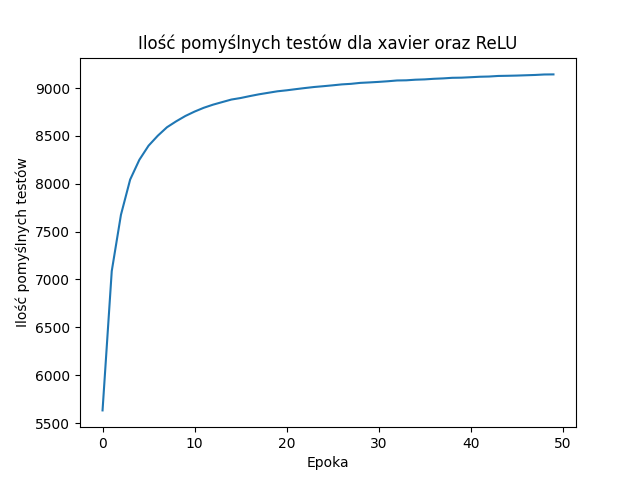
\includegraphics[width=\linewidth]{test_xavier_ReLU.png}
\end{figure}

W przypadku funkcji ReLU nie widać aż tak dużej zmiany jak to było w przypadku funkcji sigmoidalnej - jest ale mniej widoczna.

\newpage
\begin{figure}[!htb]
  \centering
  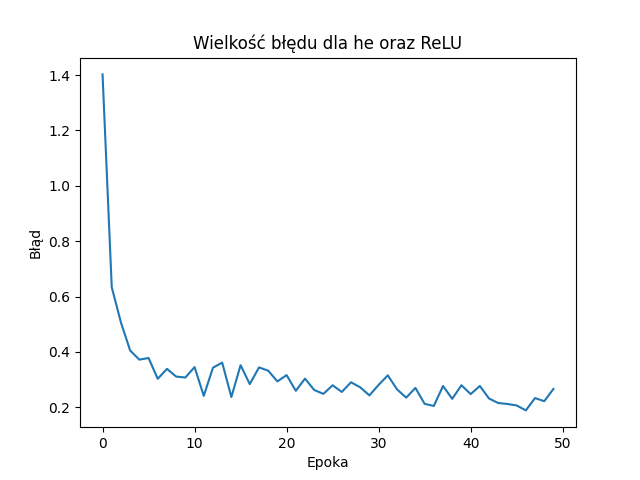
\includegraphics[width=\linewidth]{error_he_ReLU.png}
\end{figure}

\begin{figure}[!htb]
  \centering
  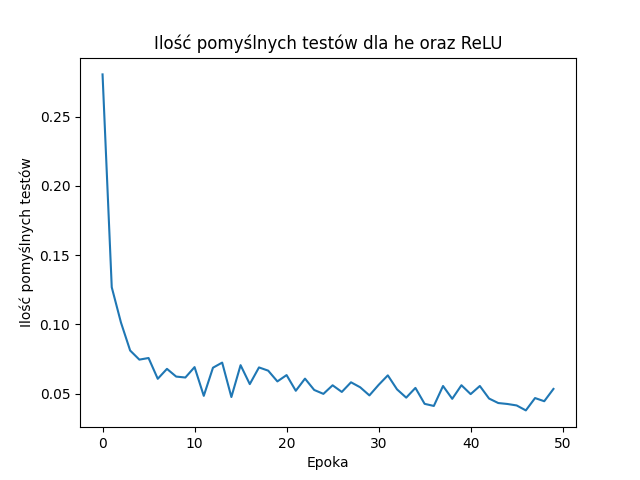
\includegraphics[width=\linewidth]{test_he_ReLU.png}
\end{figure}

Poprawa nie jest zauważalna - wyniki są na poziomie metody xaviera.

\section{Wnioski}

\subsection{Optymaliztory współczynnika uczenia}

Dobranie współczynnika uczenia nie jest prostym zadaniem - jeśli jest zbyt duży proces uczenia może okzać się niezbieżny.
Zbyt mały z kolei może skutkować bardzo wolnym uczeniem się sieci. Największy wpływ na dobór współczynnika uczenia ma kształt funkcji kosztu,
a ten jest bardzo zmienny. Należy zatem dostosować ten współczynnik w trakcie uczenia.

Momentum pomaga metodzie SGD na wyjście z minimum lokalnego biorąc pod uwagę prędkość w poprzednim kroku.
Momentum Nesterova dodatkowo bierze pod uwagę przewidywanie następnej pozycji.
Adagrad zmienia współczynnik uczenia w zależności od parametrów - sumuje kwadraty wszystkich gradientów.
Adadelta ogranicza sumowanie gradientów do pewnego rozmiaru.
Adam używa zarówno poprzednich gradientów, jak i przeszłych kwadratów gradientów.

Eksperymenty wskazują, że wszystkie optymalizatory znacząco ulepszają prędkość jak i skuteczność nauki sieci. 
Najlepsze wyniki osiąga optymalizator Adam.


\subsection{Metody inicjalizacji wag}

Jest bardzo istotne aby podczas projektowania sieci neuronowej wziąć pod uwagę sposób inicjalizacji wag. Inicjalizacja wag jest
punktem początkowym uczenia i może zaważyć na skuteczności sieci. Złe dobranie wag może pogorszyć skuteczność sieci, a nawet uniemożliwić naukę.
Zbyt niskie wagi mogą potencjalnie bardzo spowolnić uczenie sieci - problem zanikającego gradientu. Z kolei zbyt wysoka inicjalizacja może
skutkować bardzo dużymi liczbami w trakcie uczenia, które będą powodowały przekroczenie zakresu liczb w komputerze - problem wybuchającego gradientu.

Generalnie wagi powinny być inicjalizowane jako niewielkie wartości w pobliżu 0. Wybór rozkładu normalnego o odchyleniu standardowym = 0.1 jest prawidłowe.

Metoda Xaviera ma na celu zachować stałą wariancję od warstwy do warstwy w obu kierunkach, aby sieć mogła uczyć się optymalnie.

Ze względu na to, że funkcja ReLU zwraca wynik 0 dla wartości ujemnych - połowa wariancji będzie taka sama jak w przypadku metody xaviera, a połowa będzie równa 0.
Należało zatem zmodyfikować wzór, aby przyjmował liczbę wejść zmniejszoną o połowę.

Eksperymetny wskazują, że wykorzystanie wymienionych metod okazuje się być lepsze, niż teoretycznie poprawne wykorzytanie samego rozkłądu normalnego o niskim odchyleniu standardowym.
Metoda He została stworzona jako lepsza alternatywa dla metody xaviera w przypadku wykorzystania funkcji ReLU.
Wyniki eksperymentów są jednak na tym samym poziomie co metoda xaviera - badania autora wykazały lepszą skuteczność na bardzo głębokich sieciach,
dlatego tutaj poprawa może się nie uwidaczniać.


\end{document}